%!TEX root = thesis.tex

\chapter{Results}

	In this chapter we will attempt to generalize step 3 of Friedgut by way of generalizing Friedgut's Lemma 6, Lemma 7, and Lemma 8. However, we will begin the chapter with some general lattice theory results that we will need later on in the chapter.

\section{Lattice Theory}

	We are not aware of any existing proofs of these lemmas, but some of them are fairly elementary and seem to us to be broadly applicable.

	First we will prove, in three steps, that our inversion lattice (ordered by $\le_s$; Definition \ref{partial-order-s-definition}) remains a lattice when we identify two elements that are adjacent in the order $\le$ (Definition \ref{identified-lattice-definition}). Recall from Definition \ref{lattice-definition} that in order to be a lattice the join and meet must exist for every pair of elements. Therefore Lemma \ref{identified-permutation-lattice-join} proves that the join exists, Lemma \ref{identified-permutation-lattice-meet} proves that the meet exists (with similar reasoning), and Proposition \ref{proposition-identification-is-lattice} combines both lemmas to prove that our structure is indeed still a lattice.

	\begin{lemma}
		\label{identified-permutation-lattice-join}
		Let $(Y, \le)$ be a poset and let $X = S(Y)$. Let $(X, \le_s)$ be as in Definition \ref{partial-order-s-definition}. Let $\Inv$ be the inversion binary relation (Definition \ref{inversion-definition}) over $Y$, and let $\join$ and $\join^{ij}$ denote the join in $(X, \le_s)$ and $(X^{ij}, \le^{ij}_s)$ respectively. Then for any $i,j \in Y$, if $i$ is either a direct successor or a direct predecessor of $j$ according to $\le$, it holds that for all $x, y \in X^{ij}$:
		\[
			x \join y \text{ is defined} \implies x \join^{ij} y \text{ is defined}.
		\]
	\end{lemma}

	\begin{proof}
		Choose arbitrary $x, y \in X^{ij}$. Assume $x \join y$ is defined. Let $z = x \join y$. Then $z$ is an upper bound of $\{x, y\}$:
		\[
			z \ge_s x \textrm{ and } z \ge_s y.
		\]
		And $z$ is the least upper bound of $\{x, y\}$. For every $a \in X$:
		\[
			(a \ge_s x \textrm{ and } a \ge_s y) \implies z \le_s a.
		\]
		Since $x \in X^{ij}$, then $(i, j) \notin Inv_x$. Since $z \ge_s x$, then $(i, j) \notin Inv_z$, so $z \in X^{ij}$. By definition $z \ge_s x \implies z \ge^{ij}_s x$ and $z \ge_s y \implies z \ge^{ij}_s y$. Therefore $z$ is an upper bound of $\{x, y\}$ in $X^{ij}$.

		For any $a \in X^{ij}$ if $a$ is an upper bound of $\{x, y\}$ in $X^{ij}$ then clearly $a$ is also an upper bound of $\{x, y\}$ in $X$. Therefore $z \le_s a$, so $z \le^{ij}_s a$, which means $z = x \join^{ij} y$. So clearly $x \join^{ij} y$ exists.
	\end{proof}

	\begin{lemma}
		\label{identified-permutation-lattice-meet}
		Let $Y$ be an ordered set and let $X = S(Y)$. Let $(X, \le_s)$ be a lattice with $\le_s$ defined as above (Definition \ref{partial-order-s-definition}). Let $\Inv$ be the inversion binary relation over $Y$ as defined above (Definition \ref{inversion-definition}). Let $\meet$ and $\meet^{ij}$ denote the meet in $(X, \le_s)$ and $(X^{ij}, \le^{ij}_s)$ respectively. Then for any $i,j \in Y$, if $i$ is either a direct successor or a direct predecessor of $j$ according to $\le$, it holds that for all $x, y \in X^{ij}$:
		\[
			x \meet y \text{ is defined} \implies x \meet^{ij} y \text{ is defined}.
		\]
	\end{lemma}

	\begin{proof}
		Choose arbitrary $x, y \in X^{ij}$. Assume $x \meet y$ is defined. Let $z = x \meet y$. Then $z$ is a lower bound of $\{x, y\}$:
		\[
			z \le_s x \textrm{ and } z \le_s y.
		\]
		And $z$ is the greatest lower bound of $\{x, y\}$: for every $a \in X$:
		\[
			(a \le_s x \textrm{ and } a \le_s y) \implies z \ge_s a.
		\]
		We now show that $z \in X^{ij}$. Since $z = x \meet y$, it holds that $\Inv_z = (\Inv_x \cup \Inv_y)^t$ (Definition \ref{transitive-closure-definition}, Definition \ref{partial-order-s-definition}) \cite{markowsky1994permutation}. Because $x,y \in X^{ij}$ we know that $(i, j) \notin (\Inv_x \cup \Inv_y)$. Therefore, in order to have $(i, j) \in (\Inv_x \cup \Inv_y)^t$ we would need to have $(i, k) \in \Inv_x$ and $(k, j) \in \Inv_y$ for some $k \in Y$, which is impossible because $i$ is either a direct successor or a direct predecessor of $j$. Therefore $(i, j) \notin Inv_z$, so $z \in X^{ij}$.

		By definition $z \le_s x \implies z \le^{ij}_s x$ and $z \le_s y \implies z \le^{ij}_s y$. Therefore $z$ is a lower bound of $\{x, y\}$ in $X^{ij}$.

		For any $a \in X^{ij}$ if $a$ is a lower bound of $\{x, y\}$ in $X^{ij}$ then clearly $a$ is also a lower bound of $\{x, y\}$ in $X$. Therefore $z \ge_s a$, so $z \ge^{ij}_s a$, which means $z = x \meet^{ij} y$. So clearly $x \meet^{ij} y$ is defined.
	\end{proof}

	\begin{proposition}
		\label{proposition-identification-is-lattice}
		Let $Y$ be a set and let $X = S(Y)$. Let $(X, \le_s)$ be a lattice with $\le_s$ defined as above (Definition \ref{partial-order-s-definition}). Let $\Inv$ be the inversion binary relation over $Y$ as defined above (Definition \ref{inversion-definition}). Then for any $i,j \in Y$, if $i$ is either a direct successor or a direct predecessor of $j$ according to $\le_s$, it holds that $(X^{ij}, \le^{ij}_s)$ is a lattice.
	\end{proposition}

	\begin{proof}
		We know that $x \join y$ is defined and $x \meet y$ is defined because $(X, \le_s)$ is a lattice. Therefore by Lemma \ref{identified-permutation-lattice-join} and Lemma \ref{identified-permutation-lattice-meet} we have $x \join^{ij} y$ is defined and $x \meet^{ij} y$ is defined respectively. So $(X^{ij}, \le^{ij}_s)$ is a lattice, by definition of a lattice.
	\end{proof}

	Now we will show that a cross-product of lattices is also a lattice. For example, suppose we have the lattice in Figure \ref{figure-one-dimensional-lattice}. The top element is the greatest, and the arrows show the ``less than'' relationship between elements. Each column of numbers represents a ranking of alternatives ${1, 2, 3}$ in which we don't care about the relationship between alternative $1$ and $2$ so we simply replace alternative $2$ with $1$ in the ranking. All this aside though, this proof is valid for any lattice.

	\begin{figure}[ht]
		\begin{center}
			\includegraphics[width=1in]{../figures/diagram5.pdf}
			\caption{A single dimension of lattice.}
			\label{figure-one-dimensional-lattice}
		\end{center}
	\end{figure}

	If we were to make that lattice into a 2-dimensional ``grid'' it would look like Figure \ref{figure-two-dimensional-lattice}. This would be the case if we only had two voters ($n = 2$).

	\begin{figure}[ht]
		\begin{center}
			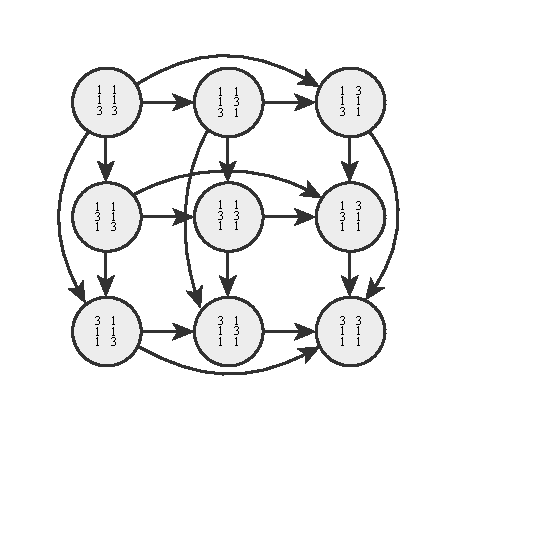
\includegraphics[width=3in]{../figures/diagram6.pdf}
			\caption{A 2-dimensional version of the lattice from Figure \ref{figure-one-dimensional-lattice}.}
			\label{figure-two-dimensional-lattice}
		\end{center}
	\end{figure}

	\begin{proposition}
		\label{proposition-grid-is-lattice}
		Let $(X, \le)$ be a lattice. Let $X^n$ be the set of all $n$-tuples of elements of $X$. Let $\le^n$ be defined as: for all $x, y \in X$
		\[
			x \le^n y \iff \forall i \in \{1, \ldots, n\}, x_i \le y_i.
		\]
		Then $(X^n, \le^n)$ is a lattice.
	\end{proposition}

	\begin{proof}
		By definition of a lattice, $(X^n, \le^n)$ is a lattice if for any two elements $s, t \in S^n$, $s \join t$ is defined and $s \meet t$ is defined.

		First, we show that $s \join t$ is defined. We define $u \in X^n$ such that $u_i = s_i \join t_i$, $\forall i \in \{1, \ldots, n\}$, and we show that $u = s \join t$. Because $u_i = s_i \join t_i$, we have
		\[
			u_i \ge s_i \textrm{ and } u_i \ge s_i
		\]
		so
		\[
			u \ge^n s \textrm{ and } u \ge^n t
		\]
		meaning that $u$ is an upper bound for $s$ and $t$. Suppose there is some $v \in X^n$ which is also an upper bound for $s$ and $t$. Then $\forall i \in \{1, \ldots, n\}$ we have
		\[
			v_i \ge s_i \textrm{ and } v_i \ge t_i
		\]
		so since $u_i = s_i \join t_i$, then $u_i \le v_i$. Therefore $u \le^n v$, i.e. $u$ is the least upper bound of $\{s, t\}$.

		Second, it follows by analogy to the above proof for $s \join t$, that $s \meet t$ is defined. Therefore, $s \join t$ is defined and $s \meet t$ is defined, so $(X^n, \le^n)$ is a lattice.
	\end{proof}


\section{Main Theorem}

	Hereafter, since we refer very often to \cite{friedgut2008elections}, instead of saying for example ``Lemma 2 of Friedgut, Kalai, and Nisan'' we will often shorten it to ``Lemma 2 of Friedgut''.

	Friedgut, Kalai, and Nisan's main theorem is proved in three steps; the first two are already general, and hold for any $n, m \in N^+$. Therefore, to generalize the main theorem we need only generalize the third step, and therefore this third step is our main theorem. This step is comprised of Lemma 6, Lemma 7, and Lemma 8 which we will generalize one at a time. The lemma we will generalize is:

	\begin{lemma}[Lemma 3 of Friedgut]
		For every SCF $f$ on $3$ alternatives and every $a,b \in A$,
		\[
			M^{a,b} \le \sum_i M_i \cdot 6
		\]
	\end{lemma}

	Which we will generalize as:

	\begin{theorem}[Main Theorem]
		For every SCF $f$ on $m$ alternatives and every $a, b \in C$:
		\[
			M^{a, b}(f) \le m! \cdot \sum_i M_i(f)
		\]
	\end{theorem}

	For the rest of the proof we will fix a SCF, $f$, and two alternatives $a, b \in C$.


\section{Generalized Lemma 6 of Friedgut}

	For any preference profile $p \in P$ there are $(\frac{m!}{2})^n$ profiles $x$ such that $x|_{\{a, b\}} = p|_{\{a, b\}}$. This is because there are $m!$ possible preference lists; half of them will have the preference between $a$ and $b$ that agrees with $p|_{\{a, b\}}$ and half will disagree. This gives $\frac{m!}{2}$ possible preference lists for each voter, so there are $(\frac{m!}{2})^n$ profiles comprised of these preference lists.

	\begin{definition}
		Let $a, b \in C$ be the first two alternatives, let $p \in L(C)^n$ be a preference profile, and let $X \subseteq L(C)^n$. We define
		\begin{align*}
			A(p, X) &= \{x \in X \mid x|_{\{a,b\}} = p|_{\{a,b\}}, f(x) = a\} \\
			B(p, X) &= \{x \in X \mid x|_{\{a,b\}} = p|_{\{a,b\}}, f(x) = b\}.
		\end{align*}
		When we do not explicitly specify $X$ we assume $X = L(C)^n$:
		\begin{align*}
			A(p) &= A(p, L(C)^n) \\
			B(p) &= B(p, L(C)^n).
		\end{align*}
	\end{definition}

	Before we state Lemma \ref{friedgut-lemma-6}, recall the definition of $M^{a,b}(f)$ from Friedgut \cite{friedgut2008elections}:
	\[
		M^{a,b}(f) = \probability(f(p) = a, f(p') = b)
	\]
	where $p, p'$ are chosen at random in $L(C)^n$ with $p|_{\{a,b\}} = p'|_{\{a,b\}}$.

	Therefore we can rewrite $M^{a,b}(f)$ as follows.

	\begin{lemma}[See Lemma 6 of Friedgut]
		\label{friedgut-lemma-6}
		\[
			M^{a,b}(f) = E_{q \in L(C)^n} \left[ \frac{|A(q)|}{\left(\frac{m!}{2}\right)^n} \cdot \frac{|B(q)|}{\left(\frac{m!}{2}\right)^n} \right],
		\]
		where $q$ is chosen uniformly at random.
	\end{lemma}
	\begin{proof}
		First we fix a profile $q$. Then
		\[
			\frac{|A(q)|}{\left(\frac{m!}{2}\right)^n}
		\]
		is the probability that a randomly chosen profile, $p$, satisfying $p|_{\{a,b\}} = q|_{\{a,b\}}$ also satisfies $f(p) = a$. This is because there are $(\frac{m!}{2})^n$ profiles that agree with $q|_{\{a,b\}}$, and $|A(q)|$ is the number of those for which the outcome is $a$.

		Likewise,
		\[
			\frac{|B(q)|}{\left(\frac{m!}{2}\right)^n}
		\]
		is the probability that a randomly chosen profile, $p'$, satisfying $p'|_{\{a,b\}} = q|_{\{a,b\}}$ also satisfies $f(p') = b$.

		Since $p|_{\{a,b\}} = q|_{\{a,b\}}$ and $p'|_{\{a,b\}} = q|_{\{a,b\}}$, clearly we have that $p|_{\{a,b\}} = p'|_{\{a,b\}}$. Since $f(p) = a$ and $f(p') = b$ are independent events, the joint probability is
		\[
			\frac{|A(q)|}{\left(\frac{m!}{2}\right)^n} \cdot \frac{|B(q)|}{\left(\frac{m!}{2}\right)^n}.
		\]
	\end{proof}


\section{Generalized Lemma 7 of Friedgut}

	We now attempt to relate $M_i(f)$ to $A$ and $B$.

	Recall the ordering, $\le_s$, which was defined in Definition \ref{partial-order-s-definition}. We know that $(L(C), \le_s)$ is a lattice by the following. First, $L(C)$ is the set of all total orderings of $C$, which is isomorphic to the set of all permutations of $C$. Second, $\le_s$ is the weak Bruhat order (also known as the weak order of permutations). The weak Bruhat order applied to the set of all permutations is a lattice \cite{bjorner1984orderings}, so $(L(C), \le_s)$ is a lattice. This is useful to note now, and will be invoked to help prove Lemma \ref{friedgut-lemma-8}.

	We have defined $(L(C), \le_s)$ to be a lattice, but for the following definition, and for later in the chapter we will treat it as a graph with $L(C)$ being the set of vertices, and $\le_s$ being the set of edges, oriented so that edges go from greater nodes to lesser nodes.---

	\begin{definition}
		Let $p \in L(C)^n$. We define the \emph{upper edge border} of $A(p)$, denoted $\partial A(p)$, to be the set of directed edges whose tail is in $A(p)$ and whose head is not in $A(p)$. We will use the notation $(x_{-i}, x_i, x'_i)$ as a shorthand to denote the edge $((x_{-i},x_i), (x_{-i},x'_i))$. Formally, for all $i \in \{1, \ldots, n\}$:
			\begin{align*}
				\partial_i A(p) = \{ (x_{-i}, x_i, x'_i) \mid \hspace{1mm} & (x_{-i}, x_i) \in A(p), \\
				& (x_{-i}, x'_i) \notin A(p), \\
				& x_i|_{\{a,b\}} = x'_i|_{\{a,b\}}, \\
				& x_i <_s x'_i \}
			\end{align*}
		and
			\[
				\partial A(p) = \bigcup_j \partial_j A(p)
			\]
		We define the upper edge border of $B(p)$ analogously.
	\end{definition}

	\begin{lemma}
		\label{manipulation-per-edge-in-a}
		Let $p, p' \in L(C)^n$, and let $i \in \{1, \ldots, n\}$. Let the following conditions hold:
		\begin{align*}
			p_{-i} &= p'_{-i} \\
			p_i|_{a,b} &= p'_i|_{a,b}.
		\end{align*}
		Then each $(x_{-i}, x_i, x'_i) \in \partial_i A(p) \cup \partial_i B(p)$ corresponds to at least one successful manipulation.
	\end{lemma}

	\begin{proof}
		By definition of the upper edge border we have
		\begin{align*}
			x_i &<_s x'_i \text{ and} \\
			x_i|_{\{a,b\}} &= x'_i|_{\{a,b\}}.
		\end{align*}

		For $(x_{-i}, x_i, x'_i) \in \partial_i A(p)$, we know that $f((x_{-i}, x_i)) = a$ and $f((x_{-i}, x'_i)) = t$ for $t \in C \backslash \{a\}$. If $t \succ_{x_i} a$ then $x'_i$ is a successful manipulation of $(x_{-i}, x_i)$. Otherwise, $a \succ_{x_i} t$. If this is the case, then we know that $(a, t) \notin Inv_{x_i}$, and because $x_i <_s x'_i$ we have $(a, t) \notin Inv_{x'_i}$, which means $a \succ_{x'_i} t$. Therefore $x_i$ is a successful manipulation of $(x_{-i}, x'_i)$.

		And analogously for $(x_{-i}, x_i, x'_i) \in \partial_i B(p)$, either $x'_i$ is a successful manipulation of $(x_{-i}, x_i)$ or $x_i$ is a successful manipulation of $(x_{-i}, x'_i)$.
	\end{proof}

	We now generalize Lemma 7 of Friedgut, Kalait, and Nisan. Their original lemma is:

	\begin{lemma}[See Lemma 7 of Friedgut]
		\[
			M_i(f) \ge \frac{1}{6} 3^{-n} E_x \left[|\partial_i A(p)| + |\partial_i B(p)| \right]
		\]
	\end{lemma}

	And we generalize it as follows.

	\begin{lemma}
		\label{friedgut-lemma-7}
		\[
			M_i(f) \ge \frac{1}{m!} \left(\frac{m!}{2}\right)^{-n} E_x \left[|\partial_i A(p)| + |\partial_i B(p)| \right]
		\]
	\end{lemma}

	\begin{proof}
		Recall the definition of $M_i(f)$: given a profile $p \in P$ and a vote $p'_i \in V$ chosen uniformly at random, $M_i(f)$ is the probability that $p'_i$ is a successful manipulation of $p$ by voter $i$. Therefore to lower bound $M_i(f)$ we start with $p$ and $p'_i$ chosen uniformly at random. We can think of these as two distinct profiles, $p$ and $p'$, where $p' = (p_{-i}, p'_i)$.

		Clearly $p_{-i}|_{\{a,b\}} = p'_{-i}|_{\{a,b\}}$, but we will have $p_i|_{\{a,b\}} = p'_i|_{\{a,b\}}$ only with probability $\frac{1}{2}$, and we condition the following on this being the case. So we assume that $p|_{\{a,b\}} = p'|_{\{a,b\}}$.

		By Lemma \ref{manipulation-per-edge-in-a}, each $(x_{-i}, x_i, x'_i) \in (\partial_i A(p) \cup \partial_i B(p))$ corresponds to at least one successful manipulation. Note that if $(x_{-i}, x_i, x'_i) \in \partial_i A(p)$ then $(x_{-i}, x'_i, x_i) \notin \partial_i A(p)$.

		We take a short aside to limit our domain without losing any information. Since we have conditioned this line of reasoning such that $p|_{\{a,b\}} = p'|_{\{a,b\}}$, for any two votes $v_1, v_2 \in A(p) \cup B(p)$ we have $v_1|_{\{a,b\}} = v_2|_{\{a,b\}}$. Therefore we can define a new set
		\[
			P' = \{x \in L(C)^n \mid x|_{\{a,b\}} = p|_{\{a,b\}}\}
		\]
		and view $A(p), B(p)$, as residing in $P'$. This is because, by definition, the elements of these sets agree with $p|_{\{a,b\}}$. Clearly $|P'| = (\frac{m!}{2})^n$.

		Therefore we can lower bound $M_i(f)$ by the probability that an edge is in either $\partial_i A(p)$ or $\partial_i B(p)$. The total possible number of edges is
		\[
			\frac{m!}{2} \cdot \frac{m!}{2} \cdot \left(\frac{m!}{2}\right)^{n-1} = \frac{m!}{2}\left(\frac{m!}{2}\right)^{n}
		\]
		So the probability that a randomly chosen edge is in either $\partial_i A(p)$ or $\partial_i B(p)$ is
		\[
			\frac{2}{m!} \left(\frac{2}{m!}\right)^{n} \cdot E \left[ |\partial_i A(p)| + |\partial_i B(p)| \right]
		\]
		Note that we can sum the probabilities for $\partial_i A(p)$ and $\partial_i B(p)$ because they are disjoint by the definition of the upper edge border; an edge cannot satisfy both $(x_{-i}, x_i) \in A(p)$ and $(x_{-i}, x_i) \in B(p)$ simultaneously because if $f((x_{-i}, x_i)) = a$ then $f((x_{-i}, x_i)) \ne b$ and vice versa.

		We conditioned our analysis on $p_{-i}|_{\{a,b\}} = p'_{-i}|_{\{a,b\}}$, so our lower bound becomes
		\[
			M_i(f) \ge \frac{1}{2} \cdot \frac{2}{m!}\left(\frac{2}{m!}\right)^{n} \cdot E \left[ |\partial_i A(p)| + |\partial_i B(p)| \right].
		\]
		After simplifying, we have
		\[
			M_i(f) \ge \frac{1}{m!}\left(\frac{2}{m!}\right)^{n} \cdot E \left[ |\partial_i A(p)| + |\partial_i B(p)| \right].
		\]
	\end{proof}

	Summing over $i$ we get the following corollary.

	\begin{corollary}[See Corollary 1 of Friedgut]
		\[
			\frac{1}{m!} \cdot \left(\frac{m!}{2}\right)^{-n} E_p[|\partial A(p)| + |\partial B(p)|] \le \sum_i M_i(f)
		\]
	\end{corollary}


\section{Generalized Lemma 8 of Friedgut}

	In this section we will fix a profile $p$, and for the sake of readability we use the following shorthand notation:
	\begin{align*}
		\le^n &\equiv (\le_s)^n \\
		A &\equiv A(p) \\
		B &\equiv B(p) \\
		A(X) &\equiv A(p, X) \\
		B(X) &\equiv B(p, X).
	\end{align*}
	We also recall $(L(C)^n, \le^n)$ is our $n$-dimensional lattice, and that $A$ and $B$ reside in this space:
	\begin{align*}
		A &\subseteq L(C)^n \\
		B &\subseteq L(C)^n \\
	\end{align*}

	We now generalize Lemma 8 of Friedgut, Kalait, and Nisan. Their original lemma is:

	\begin{lemma}[See Lemma 8 of Freidgut]
		For every disjoint $A, B$ we have that
		\[
			|\partial A| + |\partial B| \ge \left( \frac{1}{3} \right)^n |A| \cdot |B|
		\]
	\end{lemma}

	Our generalization of the above lemma is Lemma \ref{friedgut-lemma-8}, but we must do a little bit of setup before we are ready to prove it. First we define an algorithm to consolidate $A$ into $A'$. We define $A'$ to be a consolidation of $A$ as follows. Let $A' = A$.

	\begin{algorithm}
		\begin{algorithmic}
			\For{$i = 1 \to n$}
				\For{$d \in L(C)^n$}
					\State $D \gets \{x \in L(C)^n \mid x_{-i} = d_{-i}\}$
					\For{$a \in A'(D)$}
						\State $a' \gets \max_{\le^n}(D \backslash A')$
						\State $A' \gets (A' \backslash \{a\}) \cup \{a'\}$ \Comment{replace $a$ with $a'$}
					\EndFor
				\EndFor
			\EndFor
		\end{algorithmic}
	\end{algorithm}

	Figure \ref{figure-algorithm-example} gives visual example which may aid in understanding the above algorithm. It shows key steps in the process on a very small two-dimensional example lattice.

	\begin{figure}[ht]
		\begin{center}
			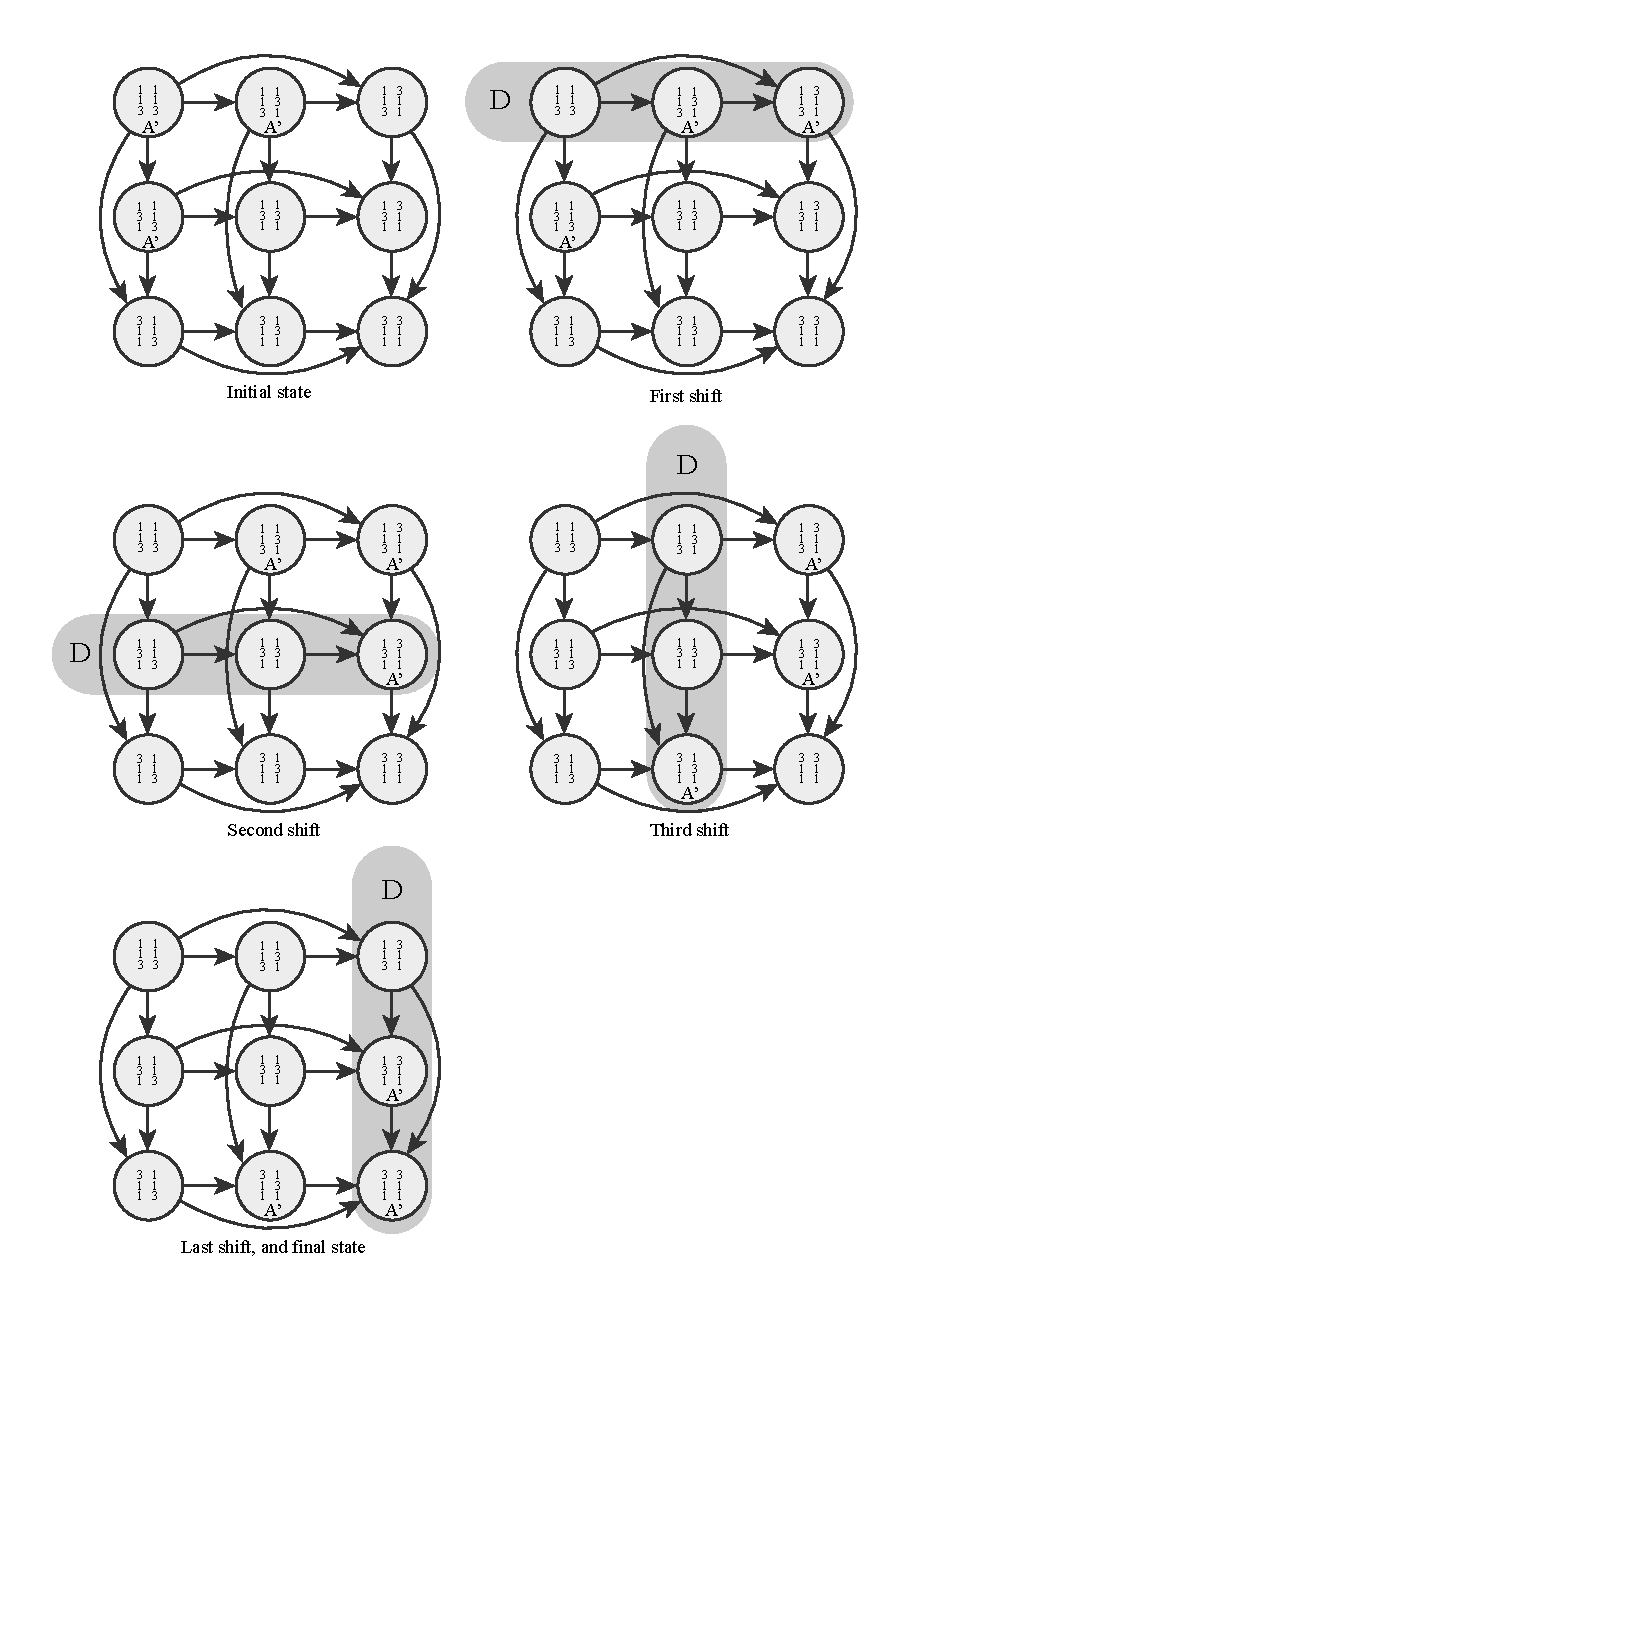
\includegraphics[width=4.6in]{../figures/diagram8.pdf}
			\caption{Example of lattice shifting algorithm.}
			\label{figure-algorithm-example}
		\end{center}
	\end{figure}

	We do the same to consolidate $B$ into $B'$.

	One of the goals of this consolidation is to achieve $A' \subseteq B'$ or $B' \subseteq A'$. While the result of this algorithm comes close to satisfying those criteria, it does not hold in all cases; see Open Problem \ref{lemma-8-open-problem}.

	\begin{openproblem}
		\label{lemma-8-open-problem}
		When using the algorithm above, we do not necessarily have $A' \subseteq B'$ or $B' \subseteq A'$. We could modify the algorithm naively so that it satisfies those criteria, but then it would become difficult to prove our second condition:
		\begin{align*}
			|A' \backslash A| &\le |\partial A| \textrm{ and} \\
			|B' \backslash B| &\le |\partial B|.
		\end{align*}
		Therefore, we leave the modification of this algorithm to achieve $A' \subseteq B'$ or $B' \subseteq A'$ as our first open problem.

		We will continue with the proof as if we do have $A' \subseteq B'$ or $B' \subseteq A'$, so that if this problem is resolved then the proof will be complete.
	\end{openproblem}

	We will now prove the following lemma.
	\begin{lemma}
		\label{lemma-8-enough-edges}
		\begin{align*}
			|A' \backslash A| &\le |\partial A| \textrm{ and} \\
			|B' \backslash B| &\le |\partial B| \\
		\end{align*}
	\end{lemma}

	\begin{proof}
		First, we show that for every $a' \in A' \backslash A$, we have an edge in $\partial A$.

		Let $a' \in A' \backslash A$. The above algorithm only adds elements to $A'$ in the innermost for loop, and since that for loop iterates once for every $a \in A(D)$ we know that for every $a'$ we have a corresponding $a$. Since $a' \in A' \backslash A$, we know that $a \ne a'$. Since $a' \gets \max_{\le^n}(A(D) \backslash A')$ and $a \ne a'$, we have that $a <^n a'$. According to the algorithm, $a, a' \in D$ which means $a_{-i} = a'_{-i}$. Therefore, $(a_{-i}, a_i, a'_i) \in \partial_i A$ by the definition of $\partial_i A$.

		Therefore, every profile in $A' \backslash A$ corresponds to at least one profile in $\partial A$, so we know that
		\[
			|A' \backslash A| \le |\partial A|.
		\]
		The same reasoning can be used to show that:
		\[
			|B' \backslash B| \le |\partial B|.
		\]
	\end{proof}

	And now we are ready to prove the final lemma in this section:

	\begin{lemma}
		\label{friedgut-lemma-8}
		For every disjoint $A, B$ we have that
		\[
			|\partial A| + |\partial B| \ge \left( \frac{2}{m!} \right)^n |A| \cdot |B|
		\]
	\end{lemma}

	\begin{proof}
		Since for any two votes $v_1, v_2 \in A \cup B$ we have $v_1|_{\{a,b\}} = v_2|_{\{a,b\}}$ we can define a new set
		\[
			P' = \{x \in P \mid x|_{\{a,b\}} = p|_{\{a,b\}}\}
		\]
		and view $A$, $B$, $A'$, and $B'$ as residing in $P'$ without losing any information. This is because, by definition, the elements of these sets agree with $p|_{\{a,b\}}$. Clearly $|P'| = (\frac{m!}{2})^n$.

		For any vote $v \in P'$, let $E_{A'}$ be the event that $v$ is in $A'$, and let $E_{B'}$ be the event that $v$ is in $B'$. Then
		\[
			P(E_{A'} \cap E_{B'}) = P(E_{A'}) P(E_{B'}|E_{A'})
		\]
		Clearly
		\begin{align}
			\label{probability-values-1}
			P(E_{A'} \cap E_{B'}) &= \frac{|A' \cap B'|}{|P'|} \\
			\label{probability-values-2}
			P(E_{A'}) &= \frac{|A'|}{|P'|} \\
			\label{probability-values-3}
			P(E_{B'}) &= \frac{|B'|}{|P'|}
		\end{align}
		Since either $A' \subseteq B'$ or $B' \subseteq A'$, we have
		\[
			P(E_{B'}|E_{A'}) \ge P(E_{B'})
		\]
		Therefore
		\[
			P(E_A \cap E_B) \ge P(E_A) P(E_B)
		\]
		So by substitution from equations \ref{probability-values-1}, \ref{probability-values-2}, and \ref{probability-values-3} we get
		\begin{align*}
			\frac{|A' \cap B'|}{(\frac{m!}{2})^n} &\ge \frac{|A'|}{(\frac{m!}{2})^n} \frac{|B'|}{(\frac{m!}{2})^n} \\
			&= \frac{|A|}{(\frac{m!}{2})^n} \frac{|B|}{(\frac{m!}{2})^n}
		\end{align*}
		However $A$ and $B$ are disjoint so
		\[
			A' \cap B' \subseteq (A' \backslash A) \cup (B' \backslash B)
		\]
		which, along with Lemma \ref{lemma-8-enough-edges}, completes the proof as follows
		\begin{align*}
			|A' \cap B'| &\le |A' \backslash A| + |B' \backslash B| \\
			|A' \cap B'| &\le |\partial A| + |\partial B| \\
			\frac{|A||B|}{(\frac{m!}{2})^n} &\le |\partial A| + |\partial B| \\
			\left(\frac{2}{m!}\right)^n |A| \cdot |B| &\le |\partial A| + |\partial B| \\
			|\partial A| + |\partial B| &\ge \left(\frac{2}{m!}\right)^n |A| \cdot |B| \\
		\end{align*}
	\end{proof}

\section{Finished Step 3 of Friedgut}

	Lemma 6, 7, and 8 fit together as follows. First we define the variables $L_6$, $L_7$, and $L_8$ to be variable values that multiply each of the lemmas respectively. The values of these variables will change depending on the value of $m$, so we evaluate the lemmas in terms of these variables to be more general. We can define the lemmas in terms of these variables:
	\begin{align*}
		&M^{a,b} = E[|A||B|] \cdot L_6 & \textrm{lemma 6} \\
		&L_7 \cdot E[|\partial A| + |\partial B|] \le \sum_i M_i & \textrm{lemma 7} \\
		&\frac{1}{L_8} \cdot (|\partial A| + |\partial B|) \ge |A||B| & \textrm{lemma 8}
	\end{align*}

	Now we can solve for the result of step 3.
	\begin{align*}
		M^{a,b} &= E[|A||B|] \cdot L_6 & \textrm{by lemma 6} \\
		M^{a,b} &\le E[|\partial A| + |\partial B|] \cdot \frac{L_6}{L_8} & \textrm{by lemma 8} \\
		M^{a,b} &\le \sum_i M_i \cdot \frac{L_6}{L_7L_8} & \textrm{by lemma 7}
	\end{align*}

	If we can fully generalize this step and capture all of the $v_i$'s our results will, possibly, look like this:
	\begin{align*}
		L_6 &= \left(\frac{m!}{2}\right)^{-2n} \\
		L_7 &= \frac{1}{m!}\left(\frac{m!}{2}\right)^{-n} \\
		L_8 &= \left(\frac{m!}{2}\right)^{-n}
	\end{align*}

	So we have that
	\begin{align*}
		\frac{L_6}{L_7L_8} &= \left(\frac{m!}{2}\right)^{-2n} \cdot m!\left(\frac{m!}{2}\right)^{n} \cdot \left(\frac{m!}{2}\right)^{n} \\
		&= \left(\frac{m!}{2}\right)^{-2n} \cdot m! \cdot \left(\frac{m!}{2}\right)^{2n} \\
		&= m!
	\end{align*}

	And the final result for step 3 becomes
	\begin{align*}
		M^{a,b} &\le \sum_i M_i \cdot m!
	\end{align*}

\section{Main Theorem of Friedgut}

	Now we can use the Friedgut's generalized steps 1 and 2 along with our generalized version of step 3 to prove a general version of Friedgut's main theorem. We will restate Friedgut's generalized lemmas from step 1 and 2.

	\begin{lemma}[Lemma 1 of Friedgut]
		\label{friedgut-lemma-1}
		For every fixed $m$ and $\epsilon > 0$ there exists $\delta > 0$ such that if $F = f^{\otimes \binom{m}{2}}$ is a neutral IIA GSWF over $m$ alternatives with $f : \{0,1\}^n \rightarrow \{0,1\}$, and $\Delta(f, DICT) > \epsilon$, then $F$ has probability of at least $\delta \ge (C\epsilon)^{\lfloor m/3 \rfloor}$ of not having a Generalized Condorcet Winner, where $C > 0$ is an absolute constant.
	\end{lemma}

	\begin{lemma}[Lemma 2 of Friedgut]
		\label{friedgut-lemma-2}
		For every fixed $m$ there exists $\delta > 0$ such that for all $\epsilon > 0$ the following holds. Let $f$ be a neutral SCF among $m$ alternatives such that $\Delta(f, DICT) > \epsilon$. Then for all $(a,b)$ we have $M^{a,b}(f) \ge \delta$.
	\end{lemma}

	And we restate our generalized version of Friedgut's Lemma 3.

	\begin{lemma}[Lemma 3 of Friedgut]
		\label{friedgut-lemma-3}
		For every SCF $f$ on $m$ alternatives and every $a,b \in A$, $M^{a,b} \le \sum_i M_i \cdot m!$
	\end{lemma}

	With these three lemmas we can now prove a generalized version of Friedgut's main theorem.

	\begin{theorem}[Theorem 1 of Friedgut]
		There exists a constant $C > 0$ such that for every $\epsilon > 0$ the following holds. If $f$ is a neutral SCF for $n$ voters over 3 alternatives and $\Delta(f, g) > \epsilon$ for any dictatorship $g$, then $f$ has total manipulatiblity: $\sum^n_{i=1} M_i(f) \ge \frac{(C\epsilon)^{\lfloor m/3 \rfloor}}{m!}$.
	\end{theorem}

	\begin{proof}
		Lemma \ref{friedgut-lemma-2} gives us
		\begin{align*}
			M^{a,b}(f) \ge \delta
		\end{align*}
		and by substituting the result from Lemma \ref{friedgut-lemma-1} for $\delta$ we get
		\begin{align*}
			M^{a,b}(f) &\ge \delta \ge (C\epsilon)^{\lfloor m/3 \rfloor} \\
			M^{a,b}(f) &\ge (C\epsilon)^{\lfloor m/3 \rfloor} \\
		\end{align*}
		We then relate $M^{a,b}$ to $M_i$ by Lemma \ref{friedgut-lemma-3}
		\begin{align*}
			\sum^n_{i=1} M_i(f) \cdot m! &\ge M^{a,b}(f) \ge (C\epsilon)^{\lfloor m/3 \rfloor} \\
			\sum^n_{i=1} M_i(f) \cdot m! &\ge (C\epsilon)^{\lfloor m/3 \rfloor} \\
			\sum^n_{i=1} M_i(f) &\ge \frac{(C\epsilon)^{\lfloor m/3 \rfloor}}{m!} \\
		\end{align*}
	\end{proof}
